\subsection{Packed original-law evaluation: a separately frozen implementation}
\label{sec:study119c}
The negative masking result motivates a further implementation experiment,
phase C, prospectively committed at \texttt{095936f1} after the outcomes
of phases A and B were known.  It repeats all five controls, acquisition,
reference calculations and seven timing processes afresh.  The sixth
service, fused tail (F), purchases exactly the positive-mass midpoint and
endpoint payloads required by the two-level budget, in one packed call
to the unchanged original terminal compiler at each resolution.  It then
scatters the returned values and slopes to their original state/action
identities and performs the same outward aggregation.  No duplicate
requested payload is made free.  The density, certified cut defect,
$2^{-20}$ implemented-continuation allowance, original action interval,
qualification targets and complete fallback remain unchanged.  This is
post-A/B development on the previously observed catalogue, not an unseen
validation or a retrospective alteration of either earlier experiment.

\begin{table}[t]\centering\small
\caption{Phase C: complete 32-state service times, all arms and services}
\label{tab:timing119c}
\begin{tabular}{llrrrrrr}\toprule
$\alpha$ & Representation & C & G & T & M & B & F\\\midrule
1/2 & Online & 0.1030 & 0.0767 & 0.0852 & 0.1048 & 0.1074 & 0.0794 \\
1/2 & Quadratic & 0.0586 & 0.0332 & 0.0412 & 0.0627 & 0.0621 & 0.0351 \\
1/2 & ReLU & 0.0901 & 0.0937 & 0.1215 & 0.1354 & 0.1093 & 0.0807 \\
1/2 & Hinge & 0.0823 & 0.0867 & 0.1113 & 0.1278 & 0.0998 & 0.0767 \\
1/2 & Spline & 0.0569 & 0.0319 & 0.0425 & 0.0639 & 0.0638 & 0.0358 \\
1/2 & Polynomial 2 & 0.2146 & 0.1917 & 0.1998 & 0.2165 & 0.2194 & 0.2115 \\
1/2 & Polynomial 3 & 0.2796 & 0.2520 & 0.2580 & 0.2852 & 0.2892 & 0.2516 \\
1/2 & Grid & 0.2265 & 0.1935 & 0.2057 & 0.2276 & 0.2266 & 0.2001 \\
3/4 & Online & 0.0983 & 0.0750 & 0.0753 & 0.0867 & 0.0857 & 0.0712 \\
3/4 & Quadratic & 0.0570 & 0.0334 & 0.0324 & 0.0428 & 0.0419 & 0.0296 \\
3/4 & ReLU & 0.0884 & 0.0936 & 0.1164 & 0.1207 & 0.0954 & 0.0795 \\
3/4 & Hinge & 0.0789 & 0.0872 & 0.1075 & 0.1153 & 0.0848 & 0.0720 \\
3/4 & Spline & 0.0596 & 0.0331 & 0.0330 & 0.0433 & 0.0436 & 0.0315 \\
3/4 & Polynomial 2 & 0.2154 & 0.1917 & 0.1918 & 0.2046 & 0.2106 & 0.1952 \\
3/4 & Polynomial 3 & 0.2679 & 0.2403 & 0.2450 & 0.2541 & 0.2563 & 0.2402 \\
3/4 & Grid & 0.2165 & 0.1950 & 0.2022 & 0.2040 & 0.2098 & 0.1931 \\
\bottomrule\end{tabular}
\par\smallskip\footnotesize
Medians in seconds from all seven fresh sequential processes. C: 128-bin compiled; G: geometric whole-support; T: original active tail; M: positive-tail masking with the full ladder; B: masked two-level budget; F: the same budget with one packed compiler call per resolution. Every service pays its proposal, refusals, repairs and certificates. Acquisition, actual loading and enclosing process costs are reported separately. Observed ranges and every clock are retained in the development companion.
\end{table}

\begin{figure}[t]
\centering
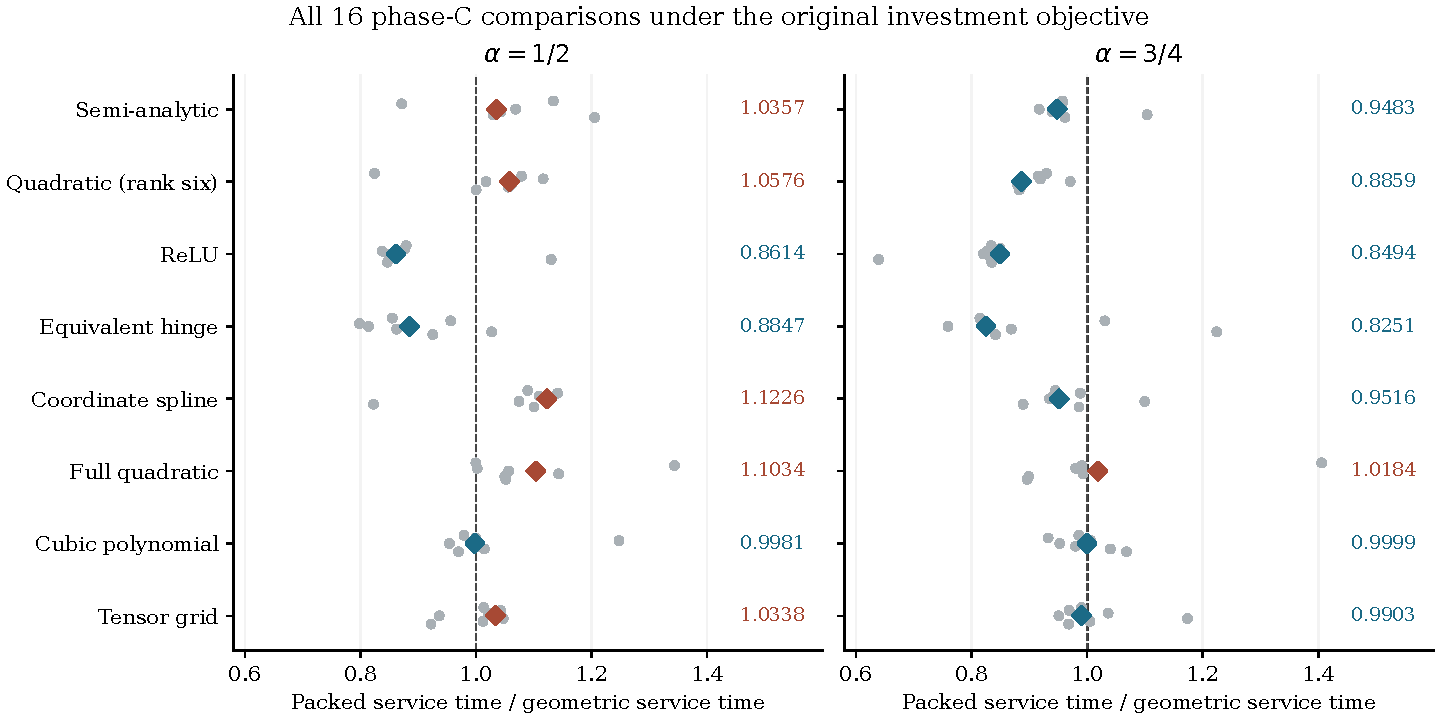
\includegraphics[width=\linewidth]{figures119/phase_c_all_clocks119.pdf}
\caption{All contemporaneous phase-C packed/geometric service comparisons.
Diamonds show the ratio of the two seven-process median times; grey points
show every paired process ratio. Values below one favor packing. These are
32-decision service clocks with actual loading and broader process costs
reported separately, not confidence intervals.}\label{fig:clocks119c}
\end{figure}

All 13,824 primary and 21,504 timing decisions completed.  The native
exact record audit passes 1,325,935 checks over 55,043 attempted
certificates; a separate read-only report verifies all 768 raw hashes
and 384,551 further exact/identity conditions.  An additional 21,974
read-only checks reconstruct the same original point coordinates for
the budgeted and fused services from their exact state, action, cut and
resolution records.  All 5,888 paired decisions use identical paid
preliminary information and qualification exits.  F uses 27 packed
compiler calls for the primary catalogue and 182 across the seven timing
processes, containing respectively 24,193 and 35,504 midpoint/endpoint
payloads.  The separate two-point defect calculation remains charged.
The 30-value general and 16-value boundary preliminary caps are attained
and respected.  Complete original risk-point queries remain 154,217,
exactly the budgeted service's count.

Table~\ref{tab:timing119c} reports the full contemporaneous comparison.
F is faster than B in all 16 median-clock cells, including 11 with all
seven paired clocks lower.  It is faster than C in all 16 medians, than
T in 14, and than G in ten.  The remaining six losses against G are
retained.  At $\alpha=1/2$, the ReLU ratio F/G is $0.8614$, with six
paired wins; at $3/4$ it is $0.8494$, with seven.  Conventional hinges
benefit similarly.  Quadratic at $1/2$ instead has ratio $1.0576$,
while quadratic at $3/4$ has ratio $0.8859$ and seven paired wins.
The degree-three polynomial ratios $0.9981$ and $0.9999$ illustrate
why a median win alone is weak evidence of a substantial advantage.
All ranges and every clock remain reported; no timing confidence
interval or architecture-independent speed guarantee is inferred.

Across all primary cells, F costs $6.5522$ seconds, compared with
$6.7726$ for G and $6.8250$ for B.  It is faster than G in 11 of 16
complete 144-state service cells and slower in five.  These totals
describe the entire predeclared tournament.  They do not construct a
new service by selecting the fastest implementation state by state.
The result identifies a practical part of the information-to-work
connection: the proved small payload budget becomes more competitive
when its many individual arrays are evaluated together.  Packing,
scattering, outward zero terms, attempted certificates and all fallback
work remain inside the measured boundary.

All fifteen within-arm service contrasts still have exactly the same
complete original policy at each of 2,304 state--risk--arm combinations.
Their original economic contrast is exactly zero.  Repacking changes
some outward endpoints---600 primary and 2,030 timing rows differ from
B---without changing their qualification exits or policies.  Original
regret and action-distance bounds retain their previous interpretation,
and no exact rational fallback is needed.  The 1,464 primary repairs
are the same 244 distinct proposals repaired under six services.

Representation-specific adoption remains unsupported.  Charging fresh
standalone acquisition and actual loading, quadratic with G costs
$0.1485$ seconds for the full $\alpha=1/2$ catalogue, versus $0.3407$
for ReLU with F.  At $3/4$, quadratic with F costs $0.1417$, versus
$0.3131$ for ReLU with F.  Quadratic also has the strictly lower
catalogue-mean original economic cost at both risks.  The ReLU--hinge
identity holds in all 96 paired files and 4,416 paired decisions,
including attempted certificates.  The conditional adoption inequality
in Section~\ref{sec:study119} therefore continues to require the full
resource and economic comparison, not an architecture label.  Phase C
adds a shared original-decision computational improvement while
preserving the negative A/B implementation findings, R97's adverse
acquisition result, and the still-open action-aligned learning and
larger-application obligations.
